\documentclass{article}

\usepackage[margin=1in]{geometry}
\usepackage[utf8]{inputenc}
\usepackage{graphicx}
\usepackage{float}
\usepackage{biblatex}
\usepackage{amsmath}
\usepackage{amsthm}
\usepackage{amssymb}
\usepackage{hyperref}
\usepackage{listings}
\usepackage{color}
\usepackage{multicol}
\usepackage{subcaption}
%\usepackage{biblatex}


\author{Carl Schiller, 9705266436}
\title{Final Project, SI1336}


\definecolor{mygreen}{rgb}{0,0.6,0}
\definecolor{mygray}{rgb}{0.5,0.5,0.5}
\definecolor{mymauve}{rgb}{0.58,0,0.82}
\definecolor{mylight}{rgb}{0.9,0.9,0.9}
\lstset{
  backgroundcolor=\color{mylight},   % choose the background color; you must add \usepackage{color} or \usepackage{xcolor}; should come as last argument
  basicstyle=\footnotesize,        % the size of the fonts that are used for the code
  breakatwhitespace=false,         % sets if automatic breaks should only happen at whitespace
  breaklines=true,                 % sets automatic line breaking
  captionpos=b,                    % sets the caption-position to bottom
  commentstyle=\color{mygreen},    % comment style
  deletekeywords={...},            % if you want to delete keywords from the given language
  escapeinside={\%*}{*)},          % if you want to add LaTeX within your code
  extendedchars=true,              % lets you use non-ASCII characters; for 8-bits encodings only, does not work with UTF-8
  frame=single,	                   % adds a frame around the code
  keepspaces=true,                 % keeps spaces in text, useful for keeping indentation of code (possibly needs columns=flexible)
  keywordstyle=\color{blue},       % keyword style
  language=C++,                 % the language of the code
  morekeywords={*,...},            % if you want to add more keywords to the set
  numbers=left,                    % where to put the line-numbers; possible values are (none, left, right)
  numbersep=5pt,                   % how far the line-numbers are from the code
  numberstyle=\tiny\color{mygray}, % the style that is used for the line-numbers
  rulecolor=\color{black},         % if not set, the frame-color may be changed on line-breaks within not-black text (e.g. comments (green here))
  showspaces=false,                % show spaces everywhere adding particular underscores; it overrides 'showstringspaces'
  showstringspaces=false,          % underline spaces within strings only
  showtabs=false,                  % show tabs within strings adding particular underscores
  stepnumber=2,                    % the step between two line-numbers. If it's 1, each line will be numbered
  stringstyle=\color{mymauve},     % string literal style
  tabsize=2,	                   % sets default tabsize to 2 spaces
  title=\lstname                   % show the filename of files included with \lstinputlisting; also try caption instead of title
}

\bibliography{report.bib}

\begin{document}
\maketitle

\section*{Abstract}
  The effects of ramp meters on freeway on ramps were studied on a simulated
  freeway in Roslags-Näsby, Sweden. Model of road was made using
  a directed graph with vertices spaced approximately every 30 meters. Cars were
  simulated by traversing the graph with a time step size of 1/60th of a second.
  No significant increase in freeway flow was noticed by deploying ramp meters
  on the on-ramp.

\tableofcontents

\newpage

\section{Introduction}
  \subsection{Problem formulation}
    This project is intended to simulate the traffic flow effect of a \textit{time fixed ramp
    meter} a freeway
    on-ramp in Roslags Näsby trafikplats, Sweden. A \textit{ramp meter} is a device that
    manages the flow of traffic onto the freeway, an example of a \textit{ramp meter} can be seen in figure \ref{pic:ramp}.
    More specifically, a \textit{time fixed ramp
    meter} that only allow one car per green signal period will be examined. There are also
    more active variants of \textit{ramp meters} which measure gaps in the traffic on the freeway
    to determine when to release vehicles, but this is beyond the scope of this project.
    Ramp metering systems have successfuly been proven to decrease congestion and
    reduce travel time on freeways.
    ~\cite{u.s._department_of_transportation_federal_highway_administration_ramp_nodate}
    \begin{figure}
      \includegraphics[width=\linewidth]{"ramp meter"}
      \caption{A typical ramp meter, image courtesy of \cite{patriarca12_english:_2008}}
      \label{pic:ramp}
    \end{figure}
  \subsection{Complex systems}
    Traffic flow is a typical example of a complex system. As described in \textit{An Introduction to Computer Simulation Methods Third Edition (revised)},
    traffic flow can be simulated by modelling the system as a \textit{Cellular Automaton}. A \textit{Cellular Automaton} is a
    grid lattice which changes state on each tick based on rules and the current configuration of the lattice. \cite{gould_introduction_nodate}
\section{Method}
  \textit{Cellular Automata} was determined to not be satisfactory when trying to model the flow of the freeway.
  This is because lane change and collision detection worked poorly on a grid lattice in two dimensions. Another
  approach was considered instead.

  \subsection{Graphs}
  \begin{multicols}{2}
    In order to model the road with several lanes, a \textit{directed graph} was
    implemented with blocks of vertices as lanes, with directed edges as paths
    for the cars to drive. In other terms, cars drive on ''rails'' and can
    only change lanes on specified vertices, as can be seen in figure \ref{pic:graph}. \cite{noauthor_gerichteter_2018}

    When using a \textit{directed graph} instead of a grid lattice, collision avoidance becomes a lot easier
    to implement. Time complexity also decreases, which improves simulation performance.
    The collision avoidance method inmplemented is $\mathcal{O}(n\cdot m^{2})$, where $n$ is the amount of cars and $m$ is the
    search area. The grid lattice as previously metioned had dimensions 550x600, which was replaced
    by a graph with approximately 140 edges which improved performance by approximately
    2000 times (if the whole system is searched for potential obstructions i.e. other cars).

    \vfill\null
    \columnbreak

    \begin{figure}[H]
      \begin{center}
        \includegraphics[width=0.8\linewidth]{"pic2"}
        \caption{Setup of road with vertices and edges.}
        \label{pic:graph}
      \end{center}
    \end{figure}
  \end{multicols}

  \subsection{Discretization}
    In contrast to \textit{Cellular Automata}
    there is no grid discretization, and thus the cars run on continuous ''tracks''.
    The distance traveled by each car is determined by the individual car's speed and
    the system wide time step size.
    Another benefit from the \textit{directed graph} implementation is that
    the directions of the cars is not required as a parameter. All that is needed in
    order to simulate a car is the speed and the distance
    to the next vertex as well as knowing which vertex the car originated from.
    When stepping in time the distance traveled is subtracted from the distance to the next vertex, and
    when the car has reached the next vertex a new target vertex is selected.

    Cars make decisions independently according to simple rules, and generates
    a complex behavior when interacting with each other i.e. braking or changing lanes.
    Some parameters are tweakable without changing the code, and each parameter
    influences the simulation in different ways.
    \subsubsection{Speed}
      The cars' speed is determined by a mean speed multiplied by a normally distributed
      variable $x \in N(1,\sigma)$, which is referred to in the code as
      ''m\_aggressiveness''. ''m\_aggressiveness'' is also involved collision detection
      and to determine when to overtake the car in front. $\sigma$ is user tweakable.
    \subsubsection{Spawn rate and car headway}
      Cars appear in two segments, either on the on-ramp or on the beginning of the freeway.
      The rate of
      which cars appear on freeways is determined by a gamma distribution
      with probability density function according to equation \ref{eq:1}. \cite{abdel-rahim_ce571:_nodate}
      \begin{equation}
        f(x) = \frac{1}{\Gamma(\alpha)\beta^{\alpha}}x^{\alpha-1}e^{-x/\beta}
        \label{eq:1}
      \end{equation}
      where $\alpha$ is the ''shape'' factor and $\beta$ is the ''rate'' factor which are
      tweakable according to which behavior is sought after. The expected mean of a
      stochastic varaiable is $\alpha\beta$, with variance $\alpha\beta^{2}$.
      This means, a larger $\beta$ implies a more spread out function.
    \subsubsection{Collision detection}
      If a car is too close to a car in front, the speed is reduced according the following rules.
      \begin{lstlisting}[language=C++]
      if (radius_to_car < ideal && delta_speed < 0 && radius_to_car > min_distance) {
          m_speed -= std::min(std::max((radius_to_car-min_distance)*0.5f,0.0f),10.0f*delta_t);
      }
      else if(radius_to_car < min_distance){
          m_speed -= std::min(std::max((min_distance-radius_to_car)*0.5f,0.0f),2.0f*delta_t);
      }
      else if(delta_speed < 0 && radius_to_car < detection_distance){
          m_speed -= std::min(
                  abs(pow(delta_speed, 2.0f)) * pow(ideal * 0.25f / radius_to_car, 2.0f) * m_aggressiveness * 0.15f,
                  10.0f * delta_t);
      }
      \end{lstlisting}
      This ensures that a car slowly approaches the car in front. The first if statement
      guarantees that it will not surpass the ''min\_distance'' distance, because the
      speed reduction follows this diverging sum.
      \begin{equation}
        d - \sum_{n = 2}^{\infty} \frac{d}{n^{2}} = 0
      \end{equation}
      where $d$ is ''radius\_to\_car-min\_distance''.
    \subsubsection{Acceleration}
      If no obstruction is in the way, a car will accelerate according to:
      \begin{lstlisting}[language=C++]
      float target = m_target_speed;
      float d_vel; // proportional control.

      if(m_speed < target*0.75){
          d_vel = m_aggressiveness*elapsed*2.0f;
      }
      else{
          d_vel = m_aggressiveness*(target-m_speed)*4*elapsed*2.0f;
      }

      m_speed += d_vel;
      \end{lstlisting}

    \subsubsection{Overtake logic and merging}
      A car decides to overtake another car if the following conditions are met.
      \begin{lstlisting}[language=C++]
          //see if we want to overtake car.

       if(closest_car != nullptr){
           //float delta_speed = closest_car->speed()-speed();
           float delta_distance = Util::distance_to_car(this,closest_car);

           if(overtake_this_car == nullptr){
               if(delta_distance > m_min_overtake_dist_trigger && delta_distance < m_max_overtake_dist_trigger && (target_speed()/closest_car->target_speed() > m_aggressiveness*1.0f ) && current_lane == 0 && closest_car->current_node->get_parent_segment()->get_lane_number(closest_car->current_node) == 0){
                   overtake_this_car = closest_car;
               }
           }

       }

       if(overtake_this_car !=nullptr){
           if(Util::is_car_behind(overtake_this_car,this) && (Util::distance_to_car(this,overtake_this_car) > m_overtake_done_dist)){
               overtake_this_car = nullptr;
           }
       }
      \end{lstlisting}
      A car will not merge if another car is occupying the lane it want to switch too.
  \subsection{Graphics rendering}
    When tweaking parameters involved in the cars' descision making, it is hard to
    get an overview of how each parameter influences the system wide behavior of the
    traffic. Thus a lot of effort has been spent on developing a graphical interface
    that shows how the traffic flows in the given configuration of parameters.
    An example of a test run is shown in the link below.
    \url{https://youtu.be/I7Jx8SScYZ8}

\section{Result}
  \subsection{Parameters}
    The following parameters have been used in the simulation.
    By varying Lane 1 $\alpha$ and Lane 2 $\alpha$ (the rate of which cars spawn on the
    freeway), the effect of a ramp meter
    on the system flow was determined. This was done by simulating the flow of different
    spawn rates with a ramp meter and without a ramp meter.
    \begin{table}[H]
      \centering
      \begin{tabular}{| l | l |}
        \hline
        Agressiveness & 1.0 \\ \hline
        Agressiveness $\sigma$ & 0.2 \\ \hline
        Global $\beta$ & 1.5 \\ \hline
        Mean speed & 20 (m/s) \\ \hline
        Lane 0 $\alpha$ & 4.0 \\ \hline
        Lane 1 $\alpha$ & 2.0 to 0.1 with step 0.1 \\ \hline
        Lane 2 $\alpha$ & 2.0 to 0.1 with step 0.1 \\ \hline
        Ramp 0 $\alpha$ & 4.0 \\ \hline
        Minimum distance to car in front & 8.0 (m) \\ \hline
        Minimum overtake distance cutoff & 10.0 (m) \\ \hline
        Maximum overtake distance cutoff & 40.0 (m) \\ \hline
        Overtake distance shutoff & 30.0 (m) \\ \hline
        Minimum merge distance & 15.0 (m) \\ \hline
        Radial search distance & 30.0 (m) \\ \hline
        Search distance forward & 50.0 (m) \\ \hline
        Time step & 1/60.0 (s) \\ \hline
        Ramp meter period & 6.0 (s) \\ \hline
      \end{tabular}
      \caption{Parameters used}
      \label{tb:1}
    \end{table}
  \subsection{Null hypothesis}
    Let $X$ be the stochastic variable associated with the mean flow of traffic
    without a ramp meter over all simulated time.
    I.e, the outcome of $X$ is the mean flow of a simulation at a given
    $\alpha$. Let $Y$ be the stochastic variable associated with the mean flow of traffic
    with a ramp meter over all simulated time. Then formulate the null hypothesis:
    \begin{equation}
      \begin{split}
        H_{0} & : X \textrm{ and } Y \textrm{ has the same distribution}\\
        H_{1} & : X\textrm{'s distribution is skewed in relation to } Y
      \end{split}
      \label{eq:null}
    \end{equation}
  \subsection{Plots}
    \begin{figure}
      \centering
      \begin{subfigure}{0.5\textwidth}
        \centering
        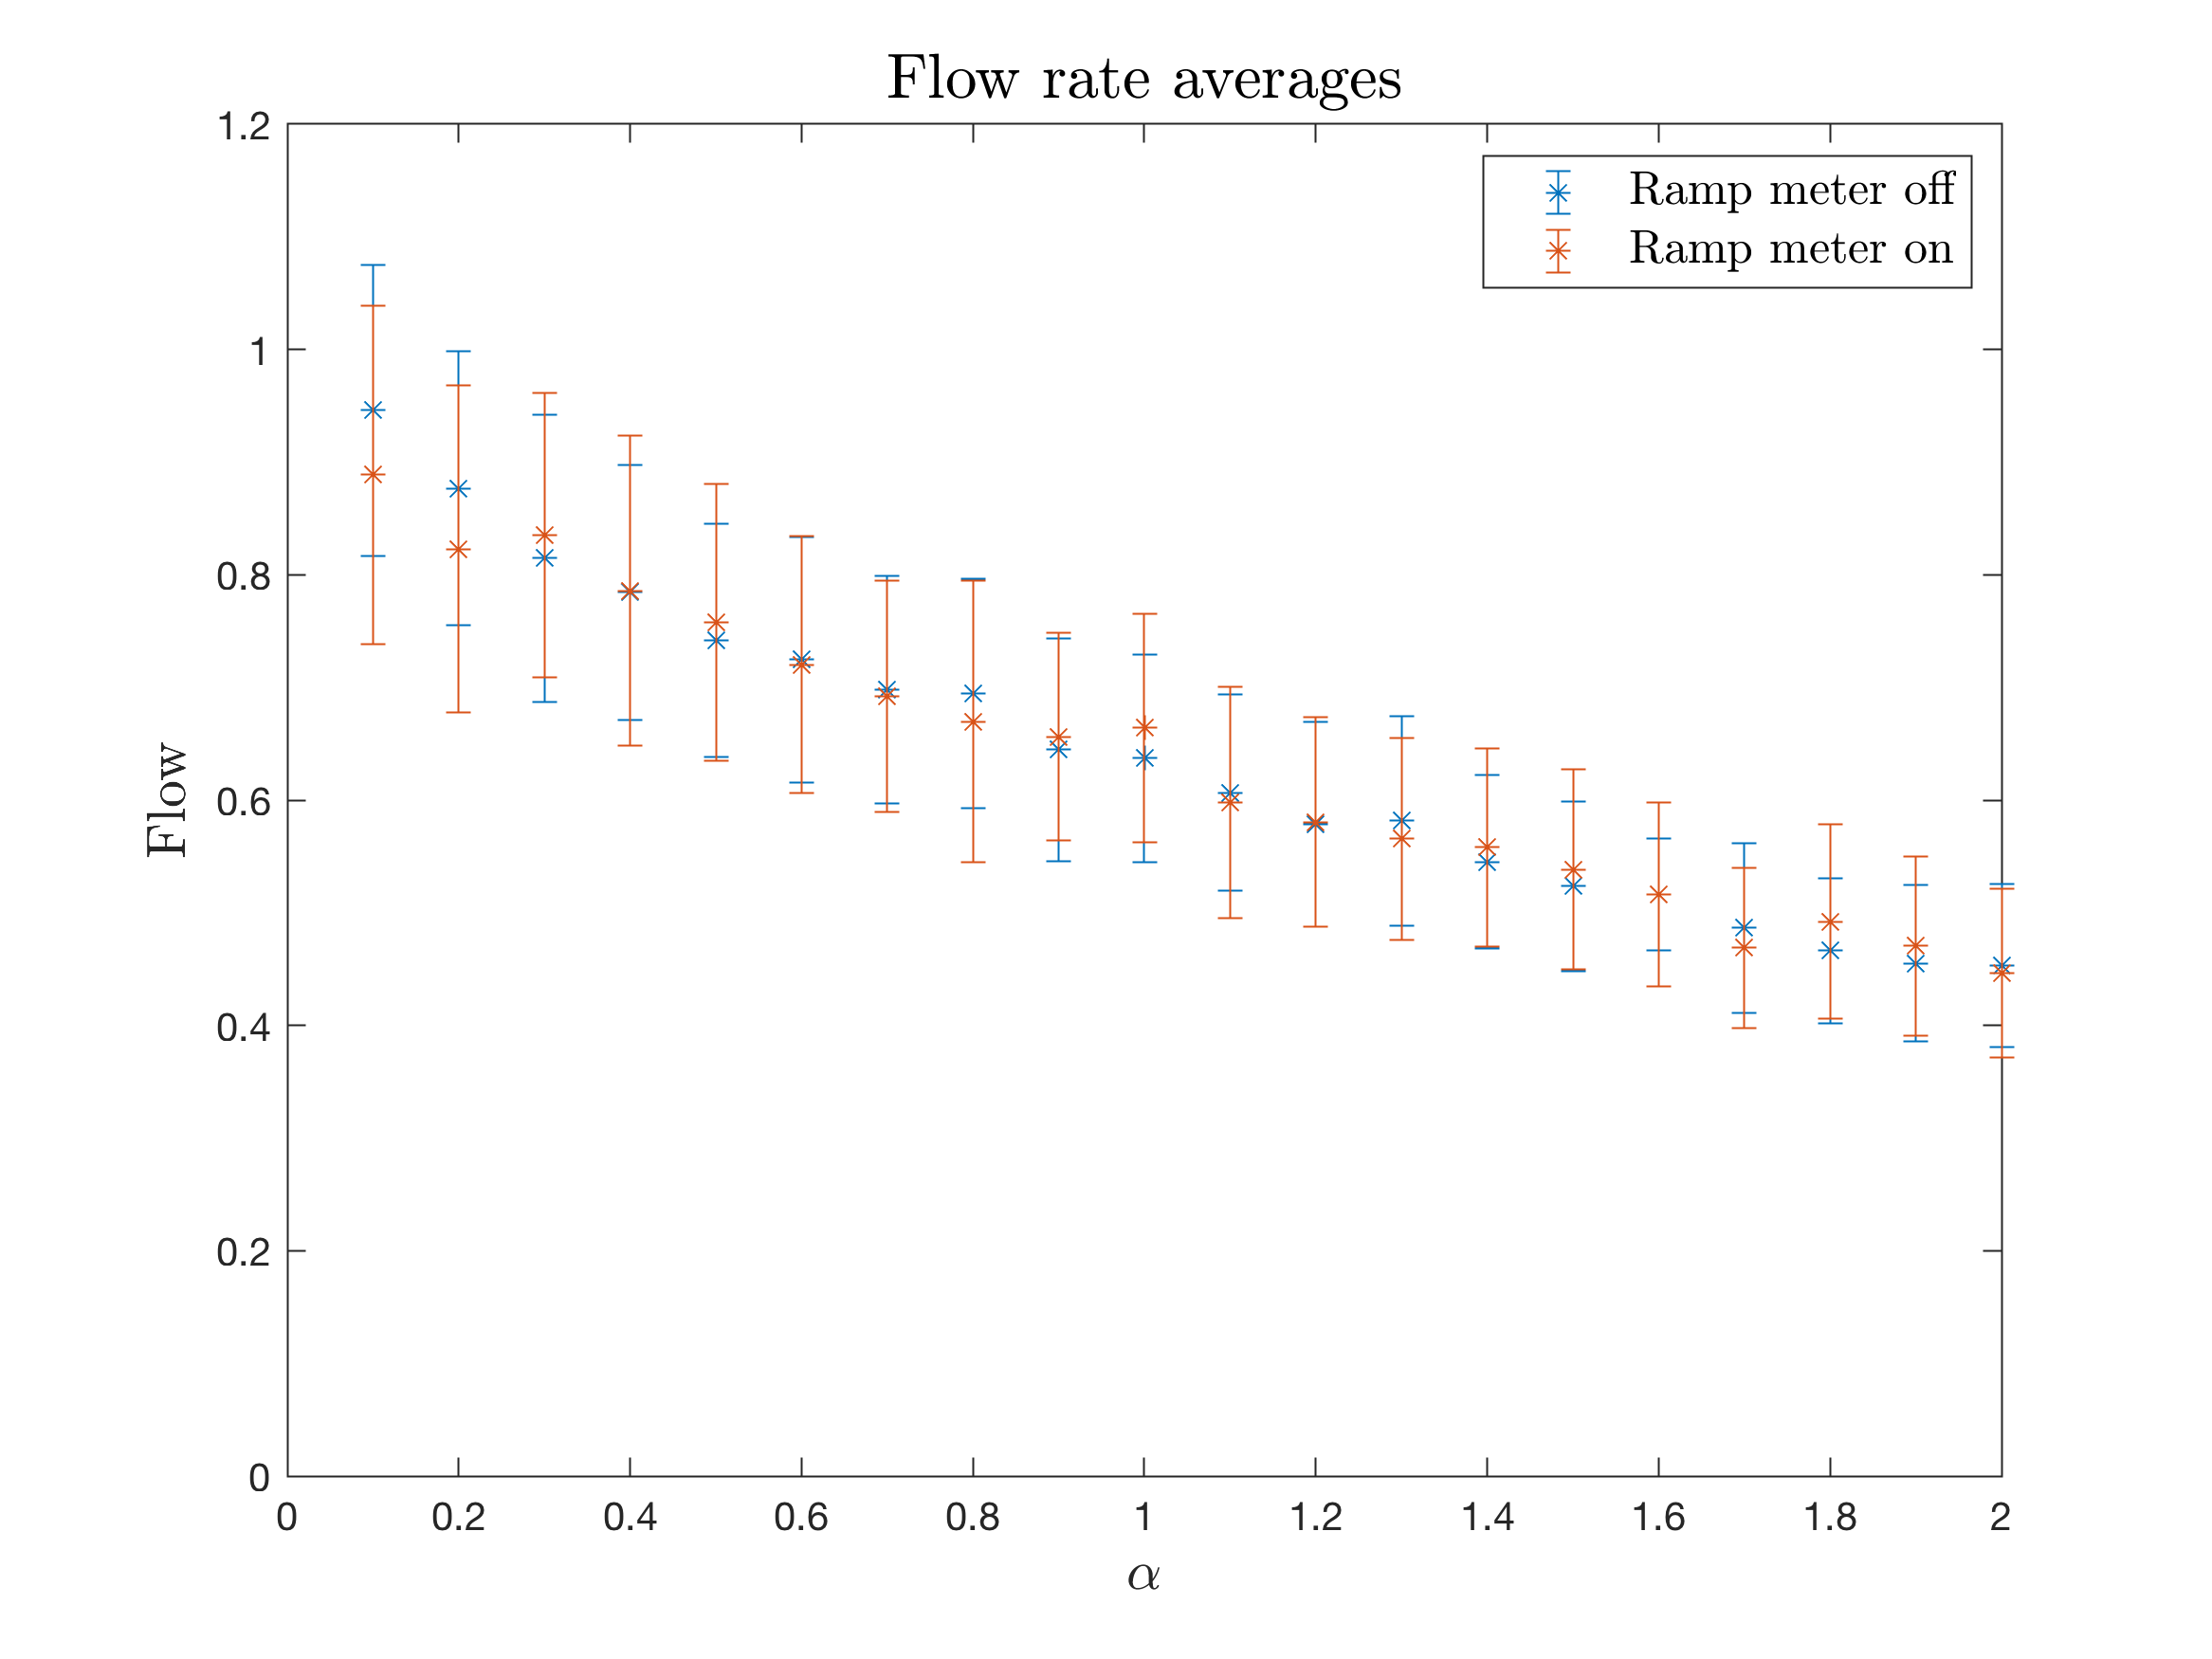
\includegraphics[width=\linewidth]{fig1.png}
        \caption{ }
        \label{sub:1}
      \end{subfigure}%
      \begin{subfigure}{0.5\textwidth}
        \centering
        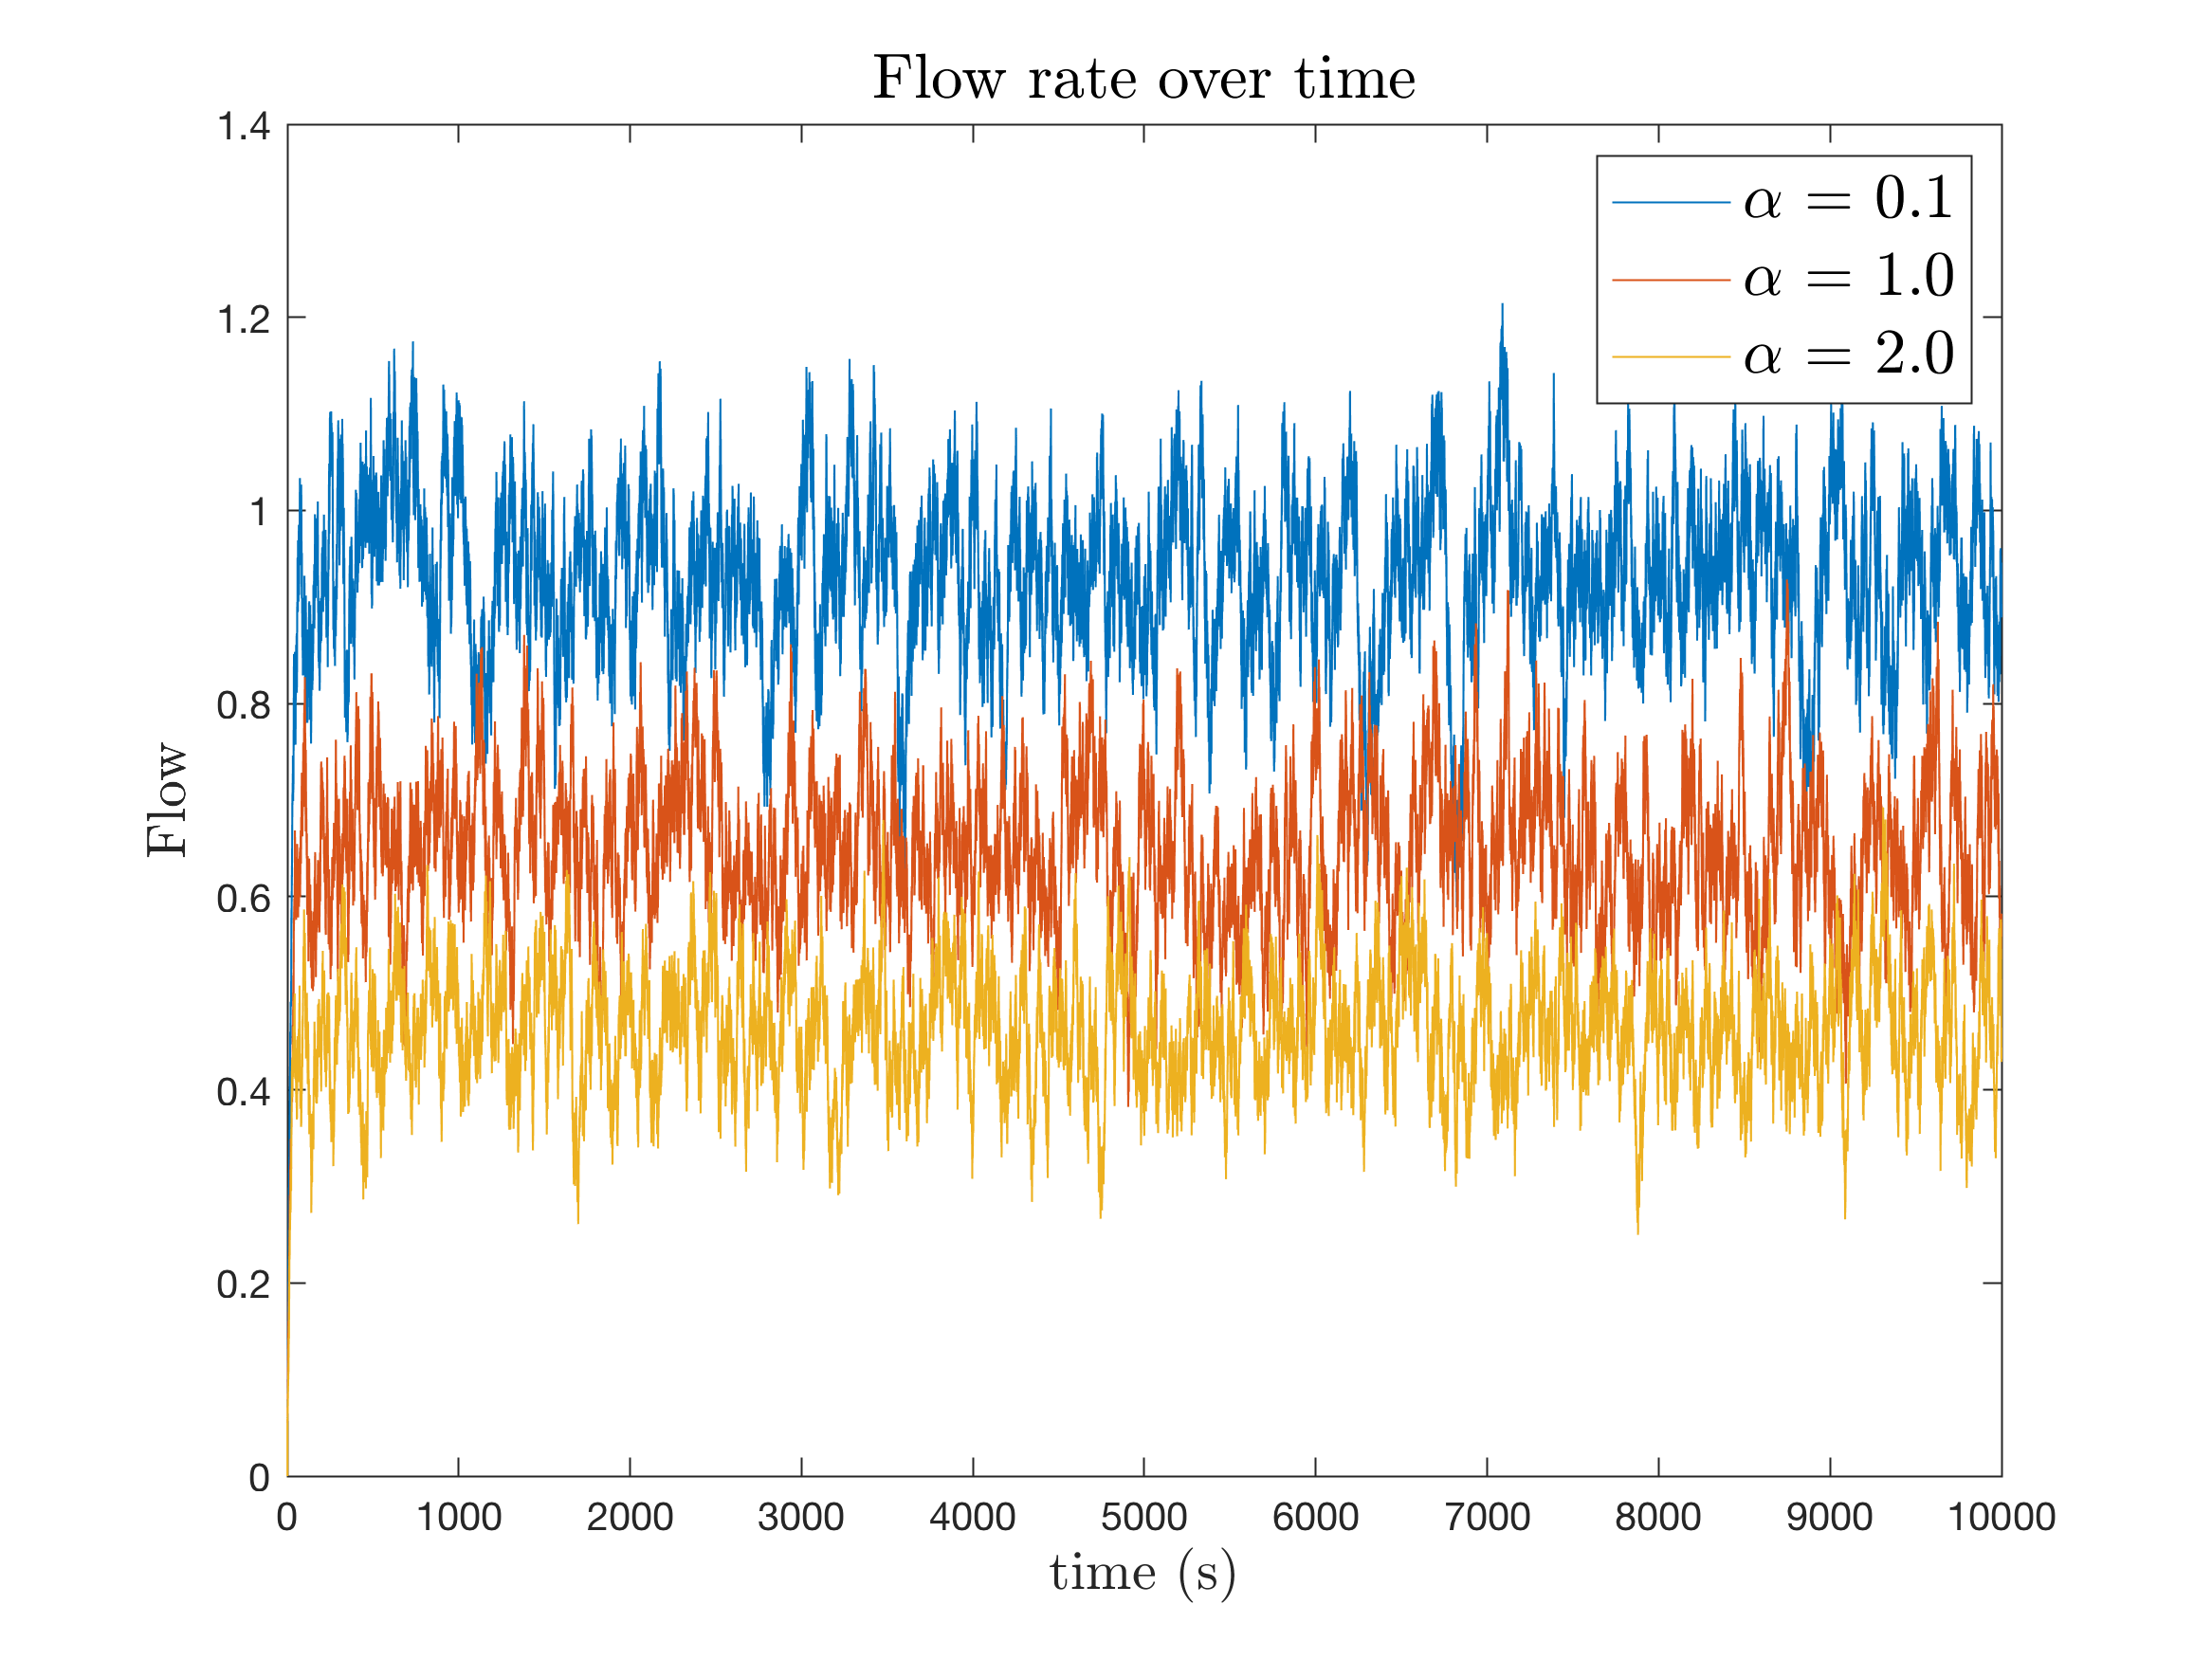
\includegraphics[width=\linewidth]{fig2.png}
        \caption{ }
        \label{sub:2}
      \end{subfigure}
      \caption{\ref{sub:1}) Fundamental diagram of flow as a function of $\alpha$ with time step 1/60 seconds. Total
      60000 steps. Errorbars represent $\pm\sigma$ of deviation in flow.
      \ref{sub:2}) Flow versus time of different $\alpha$ with time step 1/60 seconds, no ramp meter applied. Total of 600000 steps}
      \label{fig:fund}
    \end{figure}
    Figure \ref{sub:2} has characteristics typical of stop-and-go traffic for higher densities. The fluctuations of the flow
    increases as the expected spawn time $\alpha\beta$ decreases, which also can be seen by looking at figure \ref{sub:1}. The error bars
    are larger for smaller $\alpha$, which indicates a larger standard deviation from the mean flow. By using
    Wilcoxons rank sum test with equation \ref{eq:null} in mind, the p-value of the means in figure \ref{sub:1} is $p=0.9887$.
    \begin{figure}
      \centering
      \begin{subfigure}{0.33\textwidth}
        \centering
        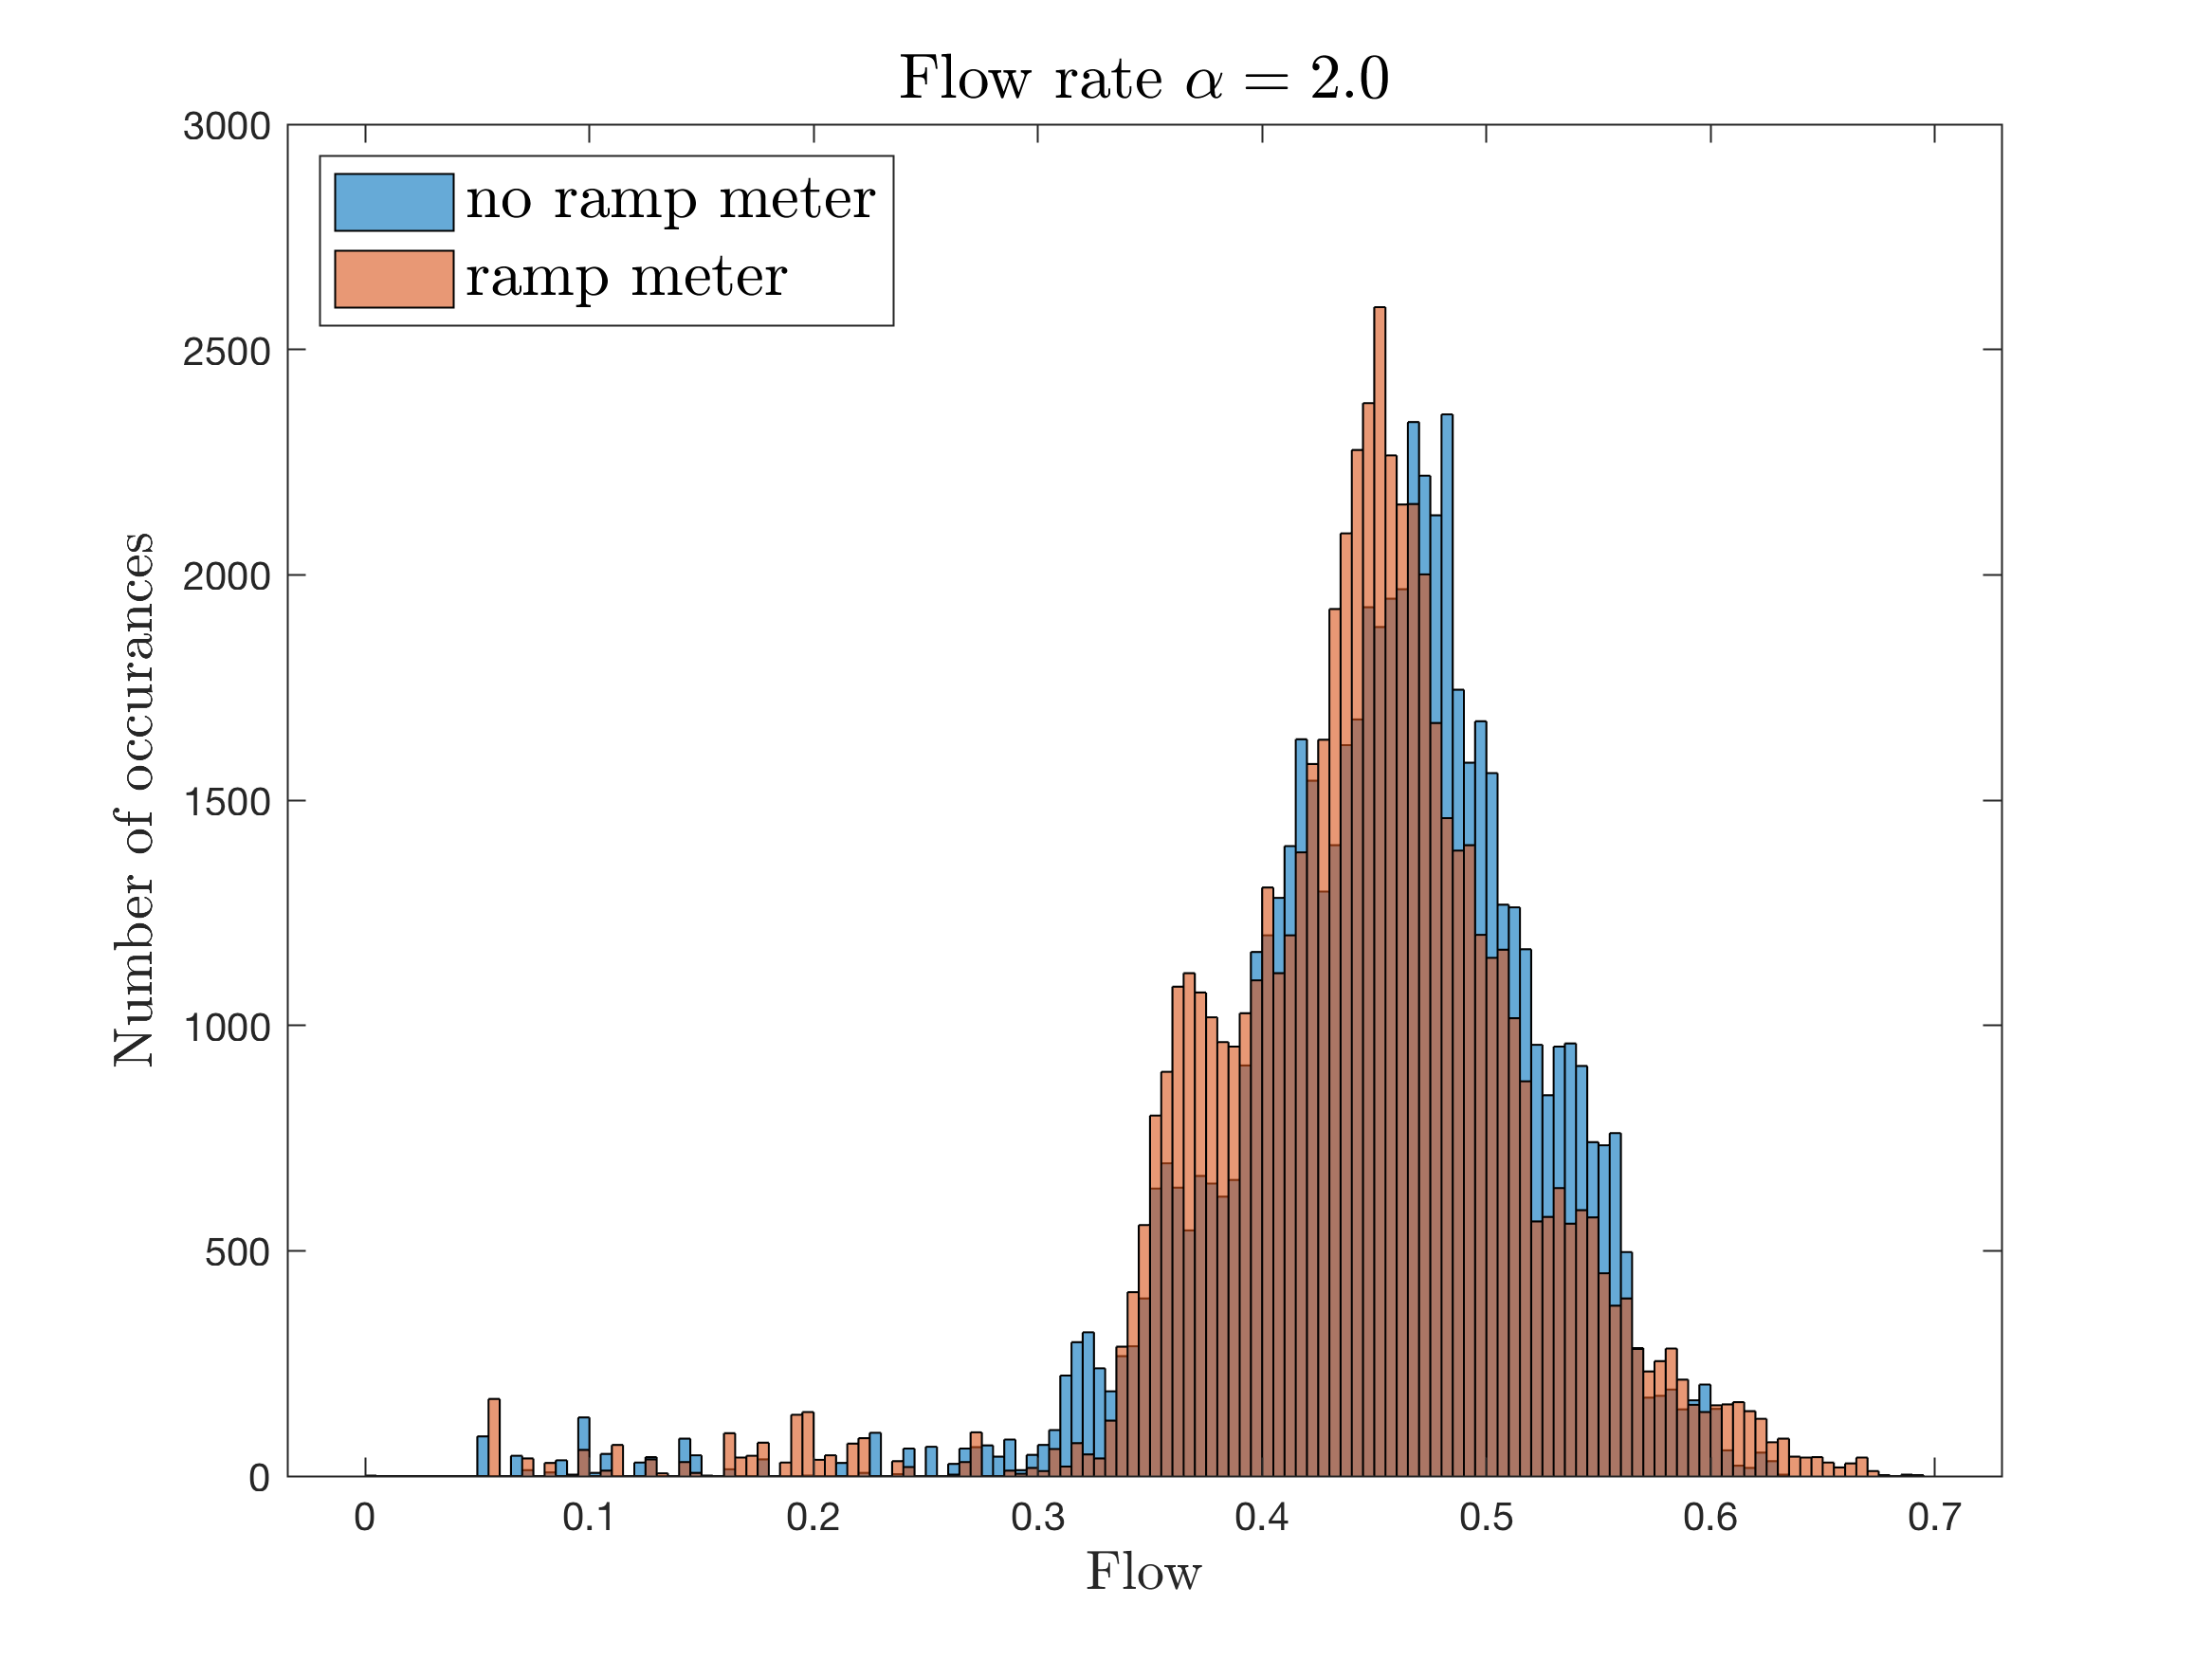
\includegraphics[width=\linewidth]{fig3.png}
        \caption{ }
        \label{sub:3}
      \end{subfigure}%
      \begin{subfigure}{0.33\textwidth}
        \centering
        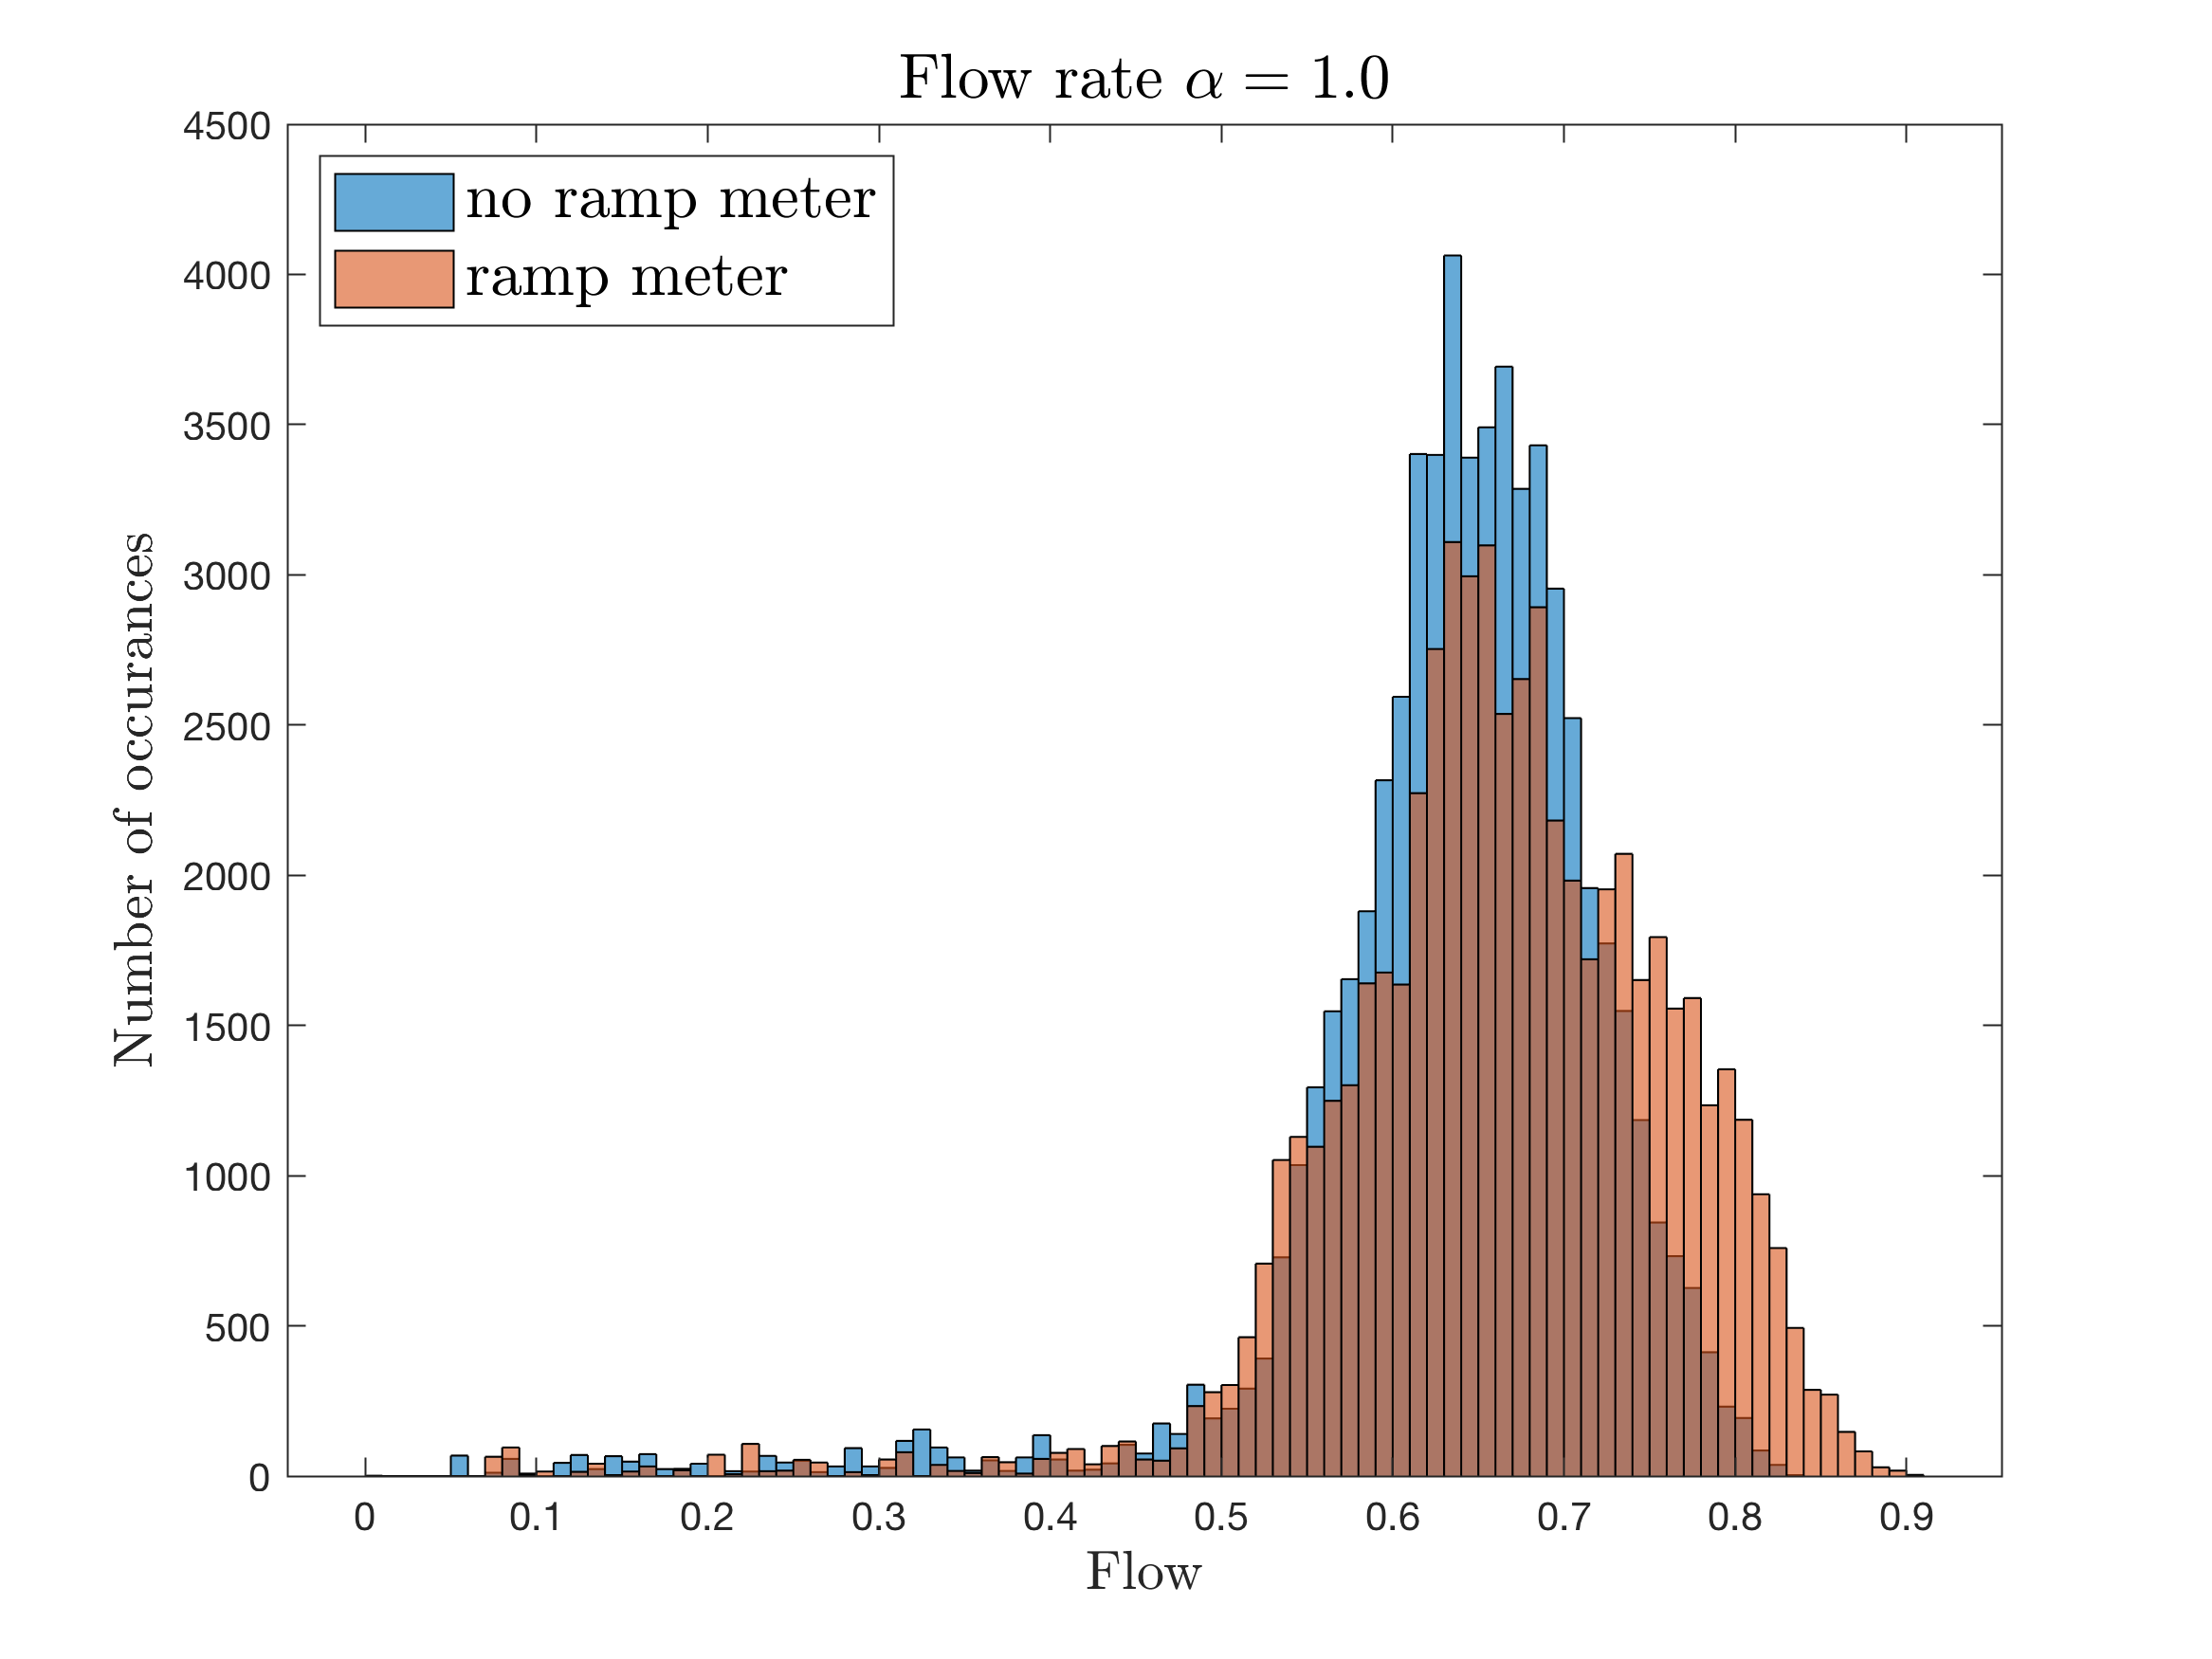
\includegraphics[width=\linewidth]{fig4.png}
        \caption{ }
        \label{sub:4}
      \end{subfigure}%
      \begin{subfigure}{0.33\textwidth}
        \centering
        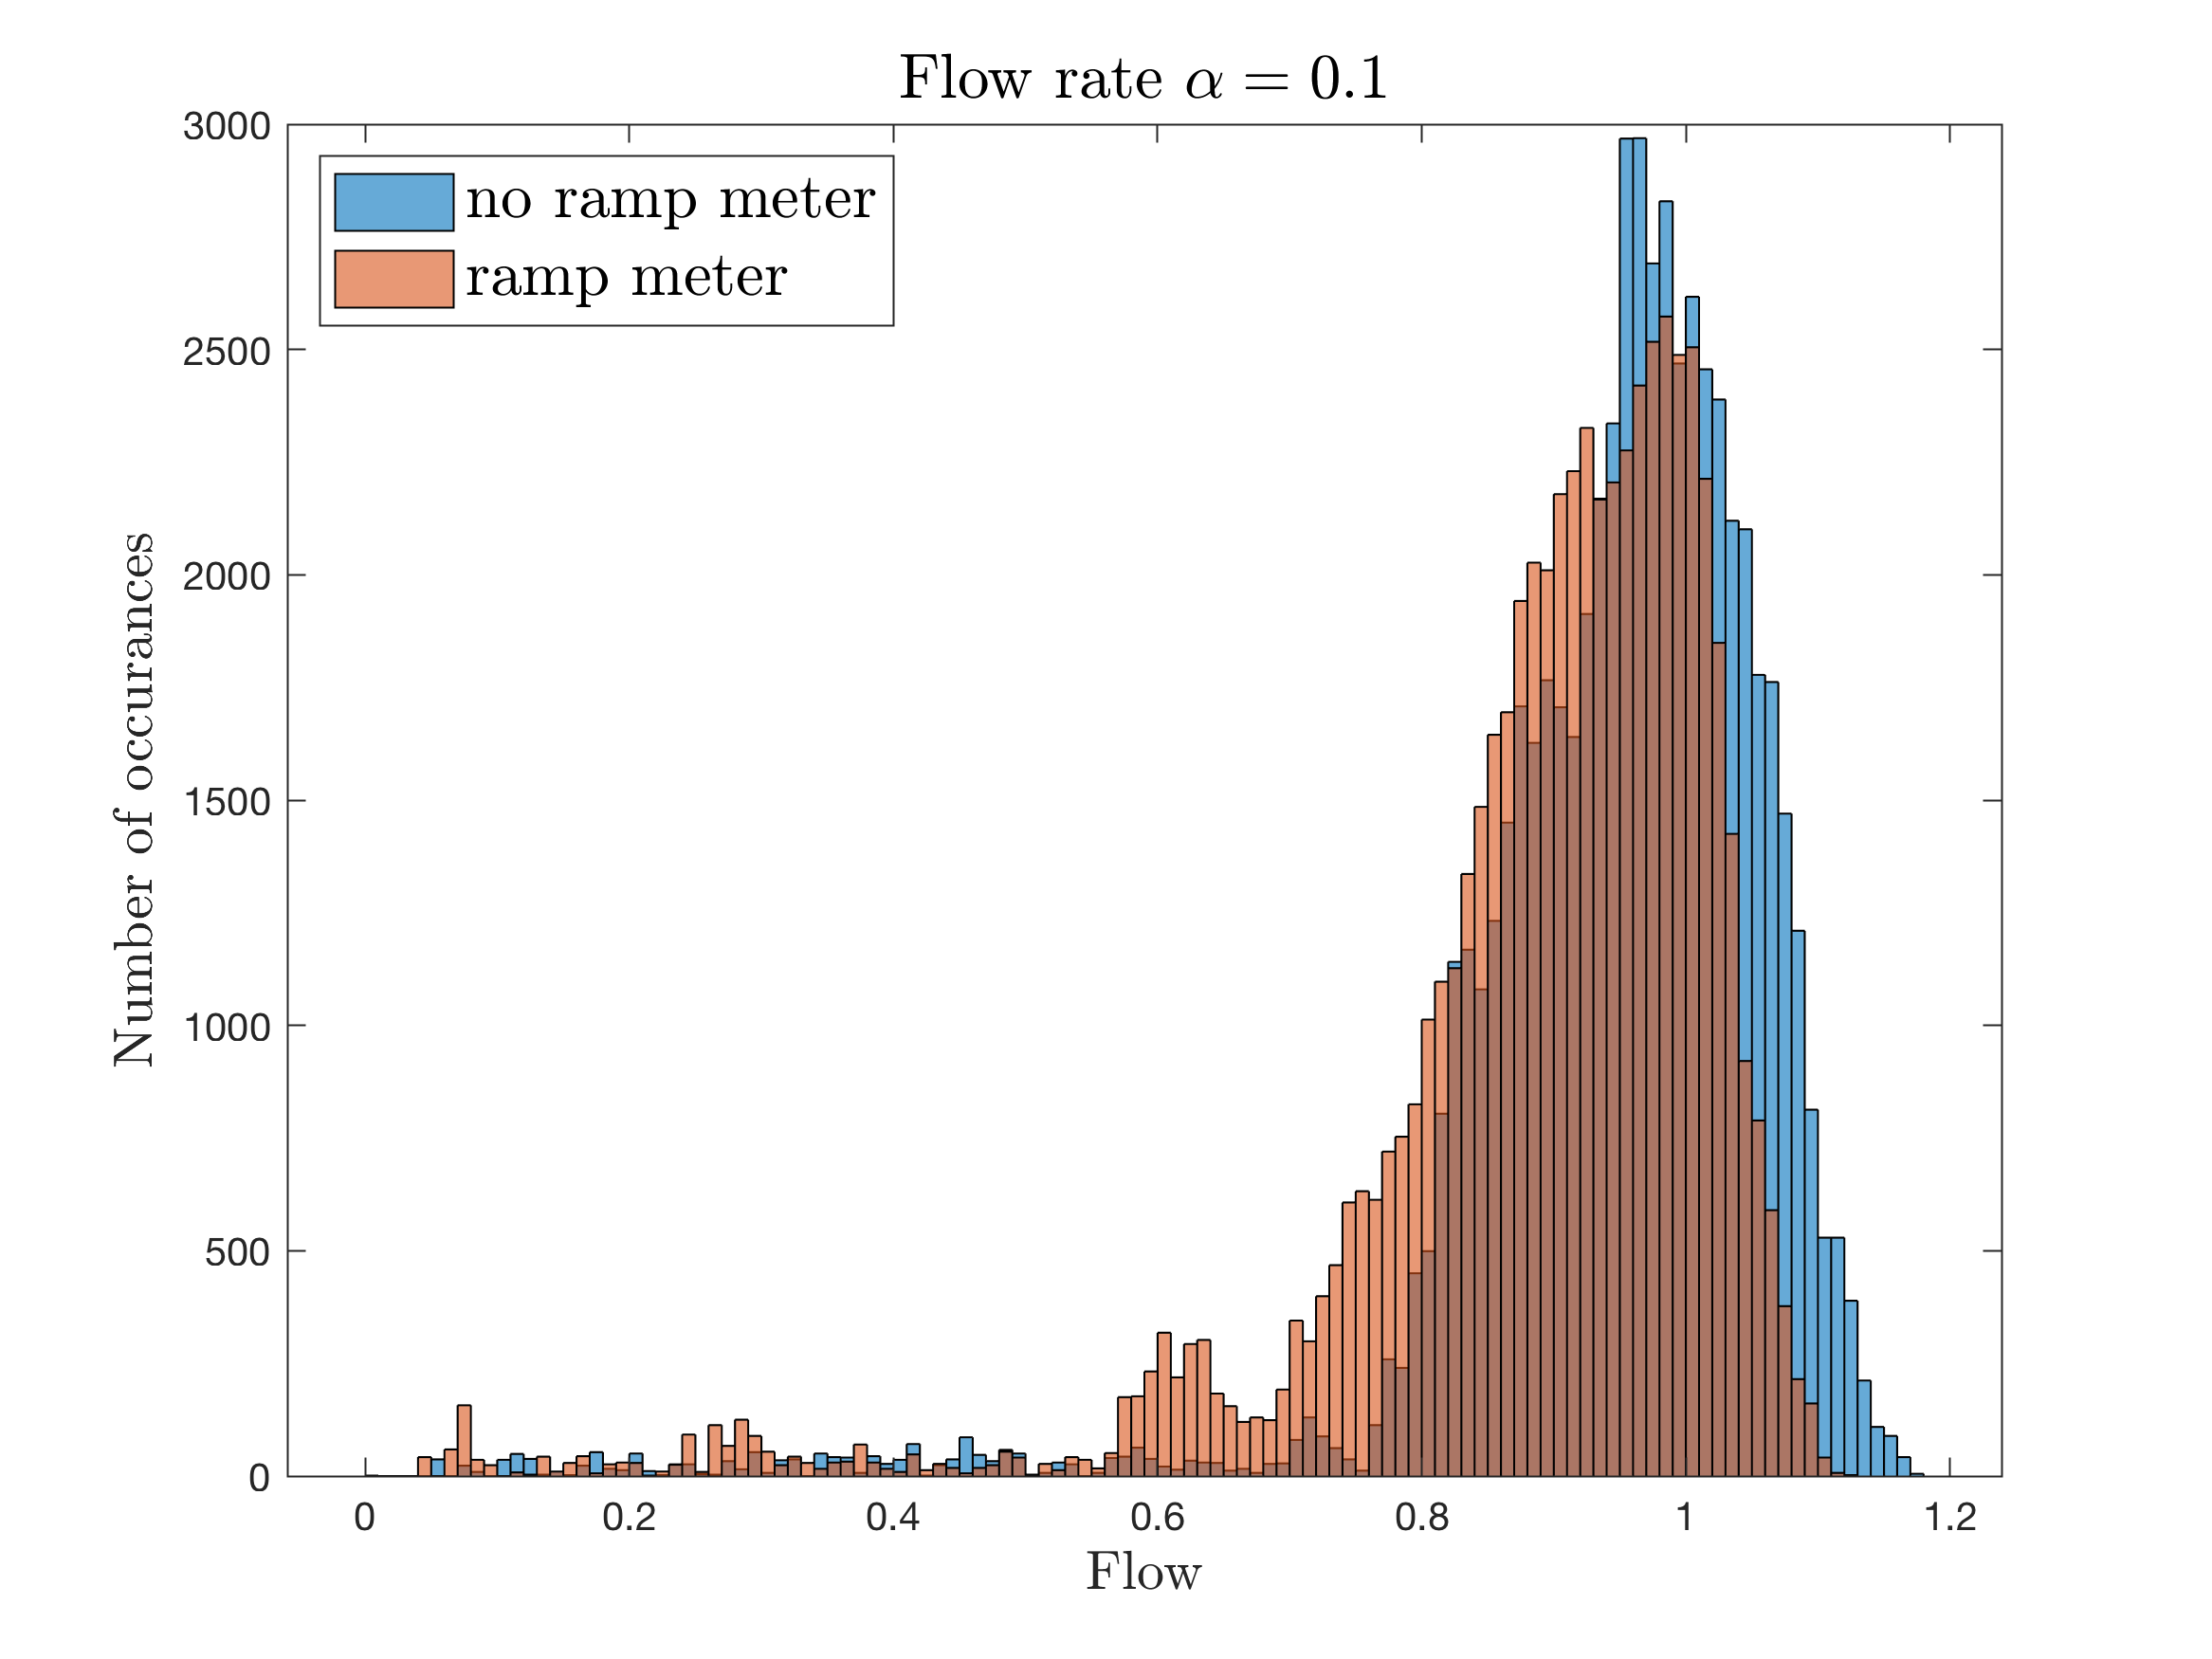
\includegraphics[width=\linewidth]{fig5.png}
        \caption{ }
        \label{sub:5}
      \end{subfigure}
      \caption{Histograms of flow for selected values of $\alpha$. Time step 1/60 seconds, total of 60000 steps}
      \label{fig:hist}
    \end{figure}
\section{Discussion}
  Since $p=0.9887 > 0.05$ the null hypothesis as formulated in equation \ref{eq:null} can not be
  rejected. I.e. there is no significant difference between using a ramp meter and not using
  a ramp meter on a 95 \% confidence level with the configuration as given in table \ref{tb:1}.
  Although for some specific values of $\alpha$ as can be seen in figure \ref{fig:hist} a
  ramp meter allows for better flow.
  \subsection{Considerations for further research}
    In this study only one parameter has been examined in table \ref{tb:1}, and
    there might be configurations where a ramp meter allows for better flow over all.
    The way cars overtake, merge, and avoid cars is also might not
    be a realistic representation of how cars behave. There might be better
    ways to model the merging, espescially in the merging segment where
    the on-ramp connects to the freeway.

    It is also worth mentioning that flow was defined as the sum of all cars divided
    by the total road length. That is, the whole system's flow was considered.
    If the flow instead was defined as the flow on the freeway only, and not the
    on-ramp, the result might have been different. This depends on what matters more,
    the total flow in the whole system or the flow on the freeway only.
\printbibliography
\pagebreak
\appendix

\section{Header files}
  \subsection{button.h}
    \lstinputlisting[language=C++]{../highway/headers/button.h}
  \subsection{cars.h}
    \lstinputlisting[language=C++]{../highway/headers/car.h}
  \subsection{cscreen.h}
    \lstinputlisting[language=C++]{../highway/headers/cscreen.h}
  \subsection{road.h}
    \lstinputlisting[language=C++]{../highway/headers/road.h}
  \subsection{roadnode.h}
    \lstinputlisting[language=C++]{../highway/headers/roadnode.h}
  \subsection{roadsegment.h}
    \lstinputlisting[language=C++]{../highway/headers/roadsegment.h}
  \subsection{screen0.h}
    \lstinputlisting[language=C++]{../highway/headers/screen0.h}
  \subsection{screen1.h}
    \lstinputlisting[language=C++]{../highway/headers/screen1.h}
  \subsection{screen2.h}
    \lstinputlisting[language=C++]{../highway/headers/screen2.h}
  \subsection{screen3.h}
    \lstinputlisting[language=C++]{../highway/headers/screen3.h}
  \subsection{screens.h}
    \lstinputlisting[language=C++]{../highway/headers/screens.h}
  \subsection{simulation.h}
    \lstinputlisting[language=C++]{../highway/headers/simulation.h}
  \subsection{simulation2.h}
    \lstinputlisting[language=C++]{../highway/headers/simulation2.h}
  \subsection{traffic.h}
    \lstinputlisting[language=C++]{../highway/headers/traffic.h}
  \subsection{unittests.h}
    \lstinputlisting[language=C++]{../highway/headers/unittests.h}
  \subsection{util.h}
    \lstinputlisting[language=C++]{../highway/headers/util.h}
\section{Source files}
  \subsection{button.cpp}
    \lstinputlisting[language=C++]{../highway/cppfiles/button.cpp}
  \subsection{cars.cpp}
    \lstinputlisting[language=C++]{../highway/cppfiles/car.cpp}
  \subsection{main.cpp}
    \lstinputlisting[language=C++]{../highway/cppfiles/main.cpp}
  \subsection{road.cpp}
    \lstinputlisting[language=C++]{../highway/cppfiles/road.cpp}
  \subsection{roadnode.cpp}
    \lstinputlisting[language=C++]{../highway/cppfiles/roadnode.cpp}
  \subsection{roadsegment.cpp}
    \lstinputlisting[language=C++]{../highway/cppfiles/roadsegment.cpp}
  \subsection{screen0.cpp}
    \lstinputlisting[language=C++]{../highway/cppfiles/screen0.cpp}
  \subsection{screen1.cpp}
    \lstinputlisting[language=C++]{../highway/cppfiles/screen1.cpp}
  \subsection{screen2.cpp}
    \lstinputlisting[language=C++]{../highway/cppfiles/screen2.cpp}
  \subsection{screen3.cpp}
    \lstinputlisting[language=C++]{../highway/cppfiles/screen3.cpp}
  \subsection{simulation.cpp}
    \lstinputlisting[language=C++]{../highway/cppfiles/simulation.cpp}
  \subsection{simulation2.cpp}
    \lstinputlisting[language=C++]{../highway/cppfiles/simulation2.cpp}
  \subsection{traffic.cpp}
    \lstinputlisting[language=C++]{../highway/cppfiles/traffic.cpp}
  \subsection{unittests.cpp}
    \lstinputlisting[language=C++]{../highway/cppfiles/unittests.cpp}
  \subsection{util.cpp}
    \lstinputlisting[language=C++]{../highway/cppfiles/util.cpp}
\section{Matlab}
  \lstinputlisting[language=Matlab]{../highway/plotter.m}
\end{document}
